\documentclass{article}
\usepackage{geometry}                % See geometry.pdf to learn the layout options. There are lots.
%\geometry{letterpaper}                   % ... or a4paper or a5paper or ...
%\geometry{landscape}                % Activate for for rotated page geometry
%\usepackage[parfill]{parIEEEabrvskip}    % Activate to begin paragraphs with an empty line rather than an indent
\usepackage{graphicx}
\usepackage{caption}
\usepackage{subcaption}
\usepackage{amssymb}
\usepackage{amsmath}
\usepackage{epstopdf}
\usepackage{amsthm}
\usepackage{authblk}
\DeclareGraphicsRule{.tif}{png}{.png}{`convert #1 `dirname #1`/`basename #1 .tif`.png}

\newtheorem*{mydef}{Definition}
\title{Determinism, Complexity, and Predictability in Computer Performance}


\author[1]{Joshua Garland \thanks{joshua.garland@colorado.edu}}
\author[1]{Ryan James \thanks{ryan.james@colorado.edu}}
\author[1,2]{Elizabeth Bradley \thanks{lizb@colorado.edu}}
\affil[1]{Department of Computer Science\\
  University of Colorado at Boulder\\
  Colorado, USA
}
\affil[2]{Santa Fe Institute\\
  New Mexico, USA
}


%Version 1
%\author{
%  \IEEEauthorblockN{Joshua Garland}
%  \IEEEauthorblockA{Dept. of Computer Science\\
%    University of Colorado at Boulder\\
%    Colorado, USA\\
%    Email: joshua.garland@colorado.edu}
%  \and
%  \IEEEauthorblockN{Ryan G.~James}
%  \IEEEauthorblockA{Complexity Sciences Center \& Dept. of Physics\\
%    University of California at Davis\\
%    California, USA\\
%    Email: rgjames@ucdavis.edu}
%    \and
%      \IEEEauthorblockN{Elizabeth Bradley}
%         \IEEEauthorblockA{Santa Fe Institute \\
%    New Mexico, USA\\
%    }
%  \IEEEauthorblockA{Dept. of Computer Science\\
%    University of Colorado at Boulder\\
%    Colorado, USA\\
%    Email: lizb@colorado.edu}
%  }



 %\author{
 %  \IEEEauthorblockN{
 %    Joshua Garland\IEEEauthorrefmark{1},
 %    Ryan G.~James\IEEEauthorrefmark{1} and
 %    Elizabeth Bradley\IEEEauthorrefmark{1}\IEEEauthorrefmark{2}}
 %  \IEEEauthorblockA{
 %    \IEEEauthorrefmark{1}Dept. of Computer Science
 %    University of Colorado, Boulder, Colorado 80309-0430 USA\\
 %    Email: joshua.garland@colorado.edu, ryan.james@colorado.edu}
 %  \IEEEauthorblockA{
 %    \IEEEauthorrefmark{2}Santa Fe Institute, 1399 Hyde Park Road, Santa Fe, New Mexico 87501  USA\\
 %    Email: lizb@colorado.edu}
 %  % \IEEEauthorblockA{
 %  %   \IEEEauthorrefmark{3}Complexity Sciences Center \& Physics Dept., University of California, Davis, %California 95616 USA\\
%   %   Email: rgjames@ucdavis.edu}
% }

\begin{document}



\maketitle





\begin{abstract}
  Computers are deterministic dynamical systems \cite{mytkowicz09}.
  Among other things, that implies that one should be able to use
  deterministic forecast rules to predict aspects of their behavior.
  That statement is sometimes---but not always---true. The memory and
  processor loads of some simple programs are easy to predict, for
  example, but those of more-complex programs like {\tt gcc} are not.
%%%%%%%%%%%%%%%%%%%%%%
%% I had to change all the \verb|blah| entries because they caused
%% latex to barf if they were in figure captions.  Odd bug.
%%%%%%%%%%%%%%%%%%%%%%
  The goal of this paper is to determine why that is the case. We
  conjecture that, in practice, complexity can effectively overwhelm
  the predictive power of deterministic forecast models. To explore
  that, we build models of a number of performance traces from
  different programs running on different Intel-based computers. We
  then calculate the \emph{permutation entropy}---a temporal entropy
  metric that uses ordinal analysis---of those traces and correlate
  those values against the prediction success.
\end{abstract}

\section{Introduction}
%\begin{it}
%Paragraph on computer performance, including citations to Todd paper
%and summary of the results that indicate that they're deterministic
%nonlinear dynamical systems.  Given that, we should be able to
%predict.  What benefits would accrue if we could do so: power mgmt,
%end world hunger [[this is my primary goal everyday :)]], etc.
%\end{it}

Computers are among the most complex engineered artifacts in current
use.  Modern microprocessor chips contain multiple processing units
and multi-layer memories, for instance, and they use complicated
hardware/software strategies to move data and threads of computation
across those resources.  These features---along with all the others
that go into the design of these chips---make the patterns of their
processor loads and memory accesses highly complex and hard to
predict.  Accurate forecasts of these quantities, if one could
construct them, could be used to improve computer design.  If one
could predict that a particular computational thread would be bogged
down for the next 0.6 seconds waiting for data from main memory, for
instance, one could save power by putting that thread on hold for that
time period (e.g., by migrating it to a processing unit whose clock
speed is scaled back).  Computer performance traces are, however, very
complex.  Even a simple ``microkernel,'' like a three-line loop that
repeatedly initializes a matrix in column-major order, can produce
{\sl chaotic} performance traces \cite{mytkowicz09}, as shown in
Figure~\ref{fig:cache}, and chaos places fundamental limits on
predictability.
%
% \begin{figure}[htbp]
%    \centering
%    \includegraphics[width=0.5\textwidth]{figs/colCacheShort}
%    % where an .eps filename suffix will be assumed under latex,
%    % and a .pdf suffix will be assumed for pdflatex
%    \caption{A small snippet of the L2 cache miss rate of {\tt
%        col\_major}, a three-line C program that repeatedly initializes
%      a matrix in column-major order, running on an Intel Core
%      Duo\textsuperscript{\textregistered}-based machine.  Even this
%      simple program exhibits chaotic performance dynamics.}
%    \label{fig:cache}
%  \end{figure}

The computer systems community has applied a variety of prediction
strategies to traces like this, most of which employ regression.  An
appealing alternative builds on the recently established fact that
computers can be effectively modeled as deterministic nonlinear
dynamical systems \cite{mytkowicz09}.  This result implies the
existence of a deterministic forecast rule for those dynamics.  In
particular, one can use \emph{delay-coordinate embedding} to
reconstruct the underlying dynamics of computer performance, then use
the resulting model to forecast the future values of computer
performance metrics such as memory or processor loads
\cite{josh-ida2011}.  In the case of simple microkernels like the one
that produced the trace in Figure~\ref{fig:cache}, this deterministic
modeling and forecast strategy works very well.  In more-complicated
programs, however, such as speech recognition software or compilers,
this forecast strategy---as well as the traditional methods---break
down quickly.

This paper is a first step in understanding when, why, and how
deterministic forecast strategies fail when they are applied to
deterministic systems.  We focus here on the specific example of
computer performance.  We conjecture that the complexity of traces
from these systems---which results from the inherent dimension,
nonlinearity, and nonstationarity of the dynamics, as well as from
measurement issues like noise, aggregation, and finite data
length---can make those deterministic signals \emph{effectively}
unpredictable.  We argue that \emph{permutation entropy}
\cite{bandt2002per}, a method for measuring the entropy of a
real-valued-finite-length time series through ordinal analysis, is an
effective way to explore that conjecture.  We study four
examples---two simple microkernels and two complex programs from the
SPEC benchmark suite---running on different Intel-based machines.  For
each program, we calculate the permutation entropy of the processor
load (instructions per cycle) and memory-use efficiency (cache-miss
rates), then compare that to the prediction accuracy attainable for
that trace using a simple deterministic model.

% paragraph to appease the theoretician in me
It is worth taking a moment to consider the theoretical possibility of
this task. We are not attempting to predict the state of the CPU at an
arbitrary point in the future --- this, at least with perfect
accuracy, would be tantamount to solving the halting problem. What we
are attempting is to predict aspects or functions of the running of
the CPU: instructions executed per second, cache misses per 100,000
instructions, and similar statistics. Prediction of these quantities
at some finite time in the future, even with perfect accuracy, does
not violate the Rice-Shapiro theorem.

% The rest of the paper is organized as follows.
% Section~\ref{sec:compModel} describes the experimental setup, as well
% as the nonlinear modeling and forecast strategies.  In
% Section~\ref{sec:meaComplex}, we review permutation entropy, calculate
% its value for a number of different computer performance traces, and
% compare the results to the prediction accuracy.  In
% Section~\ref{sec:conc}, we discuss these results and their
% implications in regard to our conjecture, and consider future areas of
% research.

\section{Modeling Computer Performance}\label{sec:compModel}

% took out for space
% \subsection{Reconstructing hidden dynamics}

Delay-coordinate embedding allows one to reconstruct a system's full
state-space dynamics from a \emph{single} scalar time-series
measurement---provided that some conditions hold regarding that data.
Specifically, if the underlying dynamics and the measurement
function---the mapping from the unknown state vector $\vec{X}$ to the
scalar value $x$ that one is measuring---are both smooth and generic,
Takens~\cite{takens} formally proves that the delay-coordinate map
\[
F(\tau,m)(x) = ([x(t) ~ x(t+\tau) ~ \dots ~x(t+m\tau)])
\]
from a $d$-dimensional smooth compact manifold $M$ to ${Re}^{2d+1}$,
where $t$ is time, is a diffeomorphism on $M$---in other words, that
the reconstructed dynamics and the true (hidden) dynamics have the
same topology.

This is an extremely powerful result: among other things, it means
that one can build a formal model of the full system dynamics without
measuring (or even knowing) every one of its state variables.  This is
the foundation of the modeling approach that is used in this paper.
The first step in the process is to estimate values for the two free
parameters in the delay-coordinate map: the delay $\tau$ and the
dimension $m$.  We follow standard procedures for this, choosing the
first minimum in the average mutual information as an estimate of
$\tau$ \cite{fraser-swinney} and using the false-near(est) neighbor
method of \cite{KBA92}, with a threshold of 10\%, to estimate $m$.  A
plot of the data from Figure~\ref{fig:cache}, embedded following this
procedure, is shown in Figure~\ref{fig:embedding}.

[[Add a plot of an embedding...]]

%% can cut for space if need be:
The coordinates of each point on this plot are differently delayed
elements of the \verb|col_major| L2 cache miss rate time series
$y(t)$: that is, $y(t)$ on the first axis, $y(t+\tau)$ on the second,
$y(t+2\tau)$ on the third, and so on.
%% ...down to here.
Structure in these kinds of plots---clearly visible in
Figure~\ref{fig:embedding}---is an indication of
determinism\footnote{A deeper analysis of
  Figure~\ref{fig:embedding}---as alluded to on the previous
  page---supports that diagnosis, confirming the presence of a chaotic
  attractor in these cache-miss dynamics, with largest Lyapunov
  exponent $\lambda_1 = 8000 \pm 200$ instructions, embedded in a
  12-dimensional reconstruction space \cite{mytkowicz09}.}.  That
structure can also be used to build a forecast model.

% took out for space
% \subsection{LMA: Using dynamics in forecasting}

Given a nonlinear model of a deterministic dynamical system in the
form of a delay-coordinate embedding like Figure~\ref{fig:embedding},
one can build deterministic forecast algorithms by capturing and
exploiting the geometry of the embedding.  Many techniques have been
developed by the dynamical systems community for this purpose
(e.g.,~\cite{casdagli-eubank92,weigend-book}).  Perhaps the most straightforward
is the ``Lorenz method of analogues'' (LMA), which is essentially
nearest-neighbor prediction in the embedded state
space~\cite{lorenz-analogues}.  Even this simple algorithm---which
builds predictions by finding the nearest neighbor in the embedded
space of the given point, then taking that neighbor's path as the
forecast---works quite well on the trace in Figure~\ref{fig:cache}, as
shown in Figure~\ref{fig:cachePredTS}.
%
\begin{figure}[htbp]
  \centering
    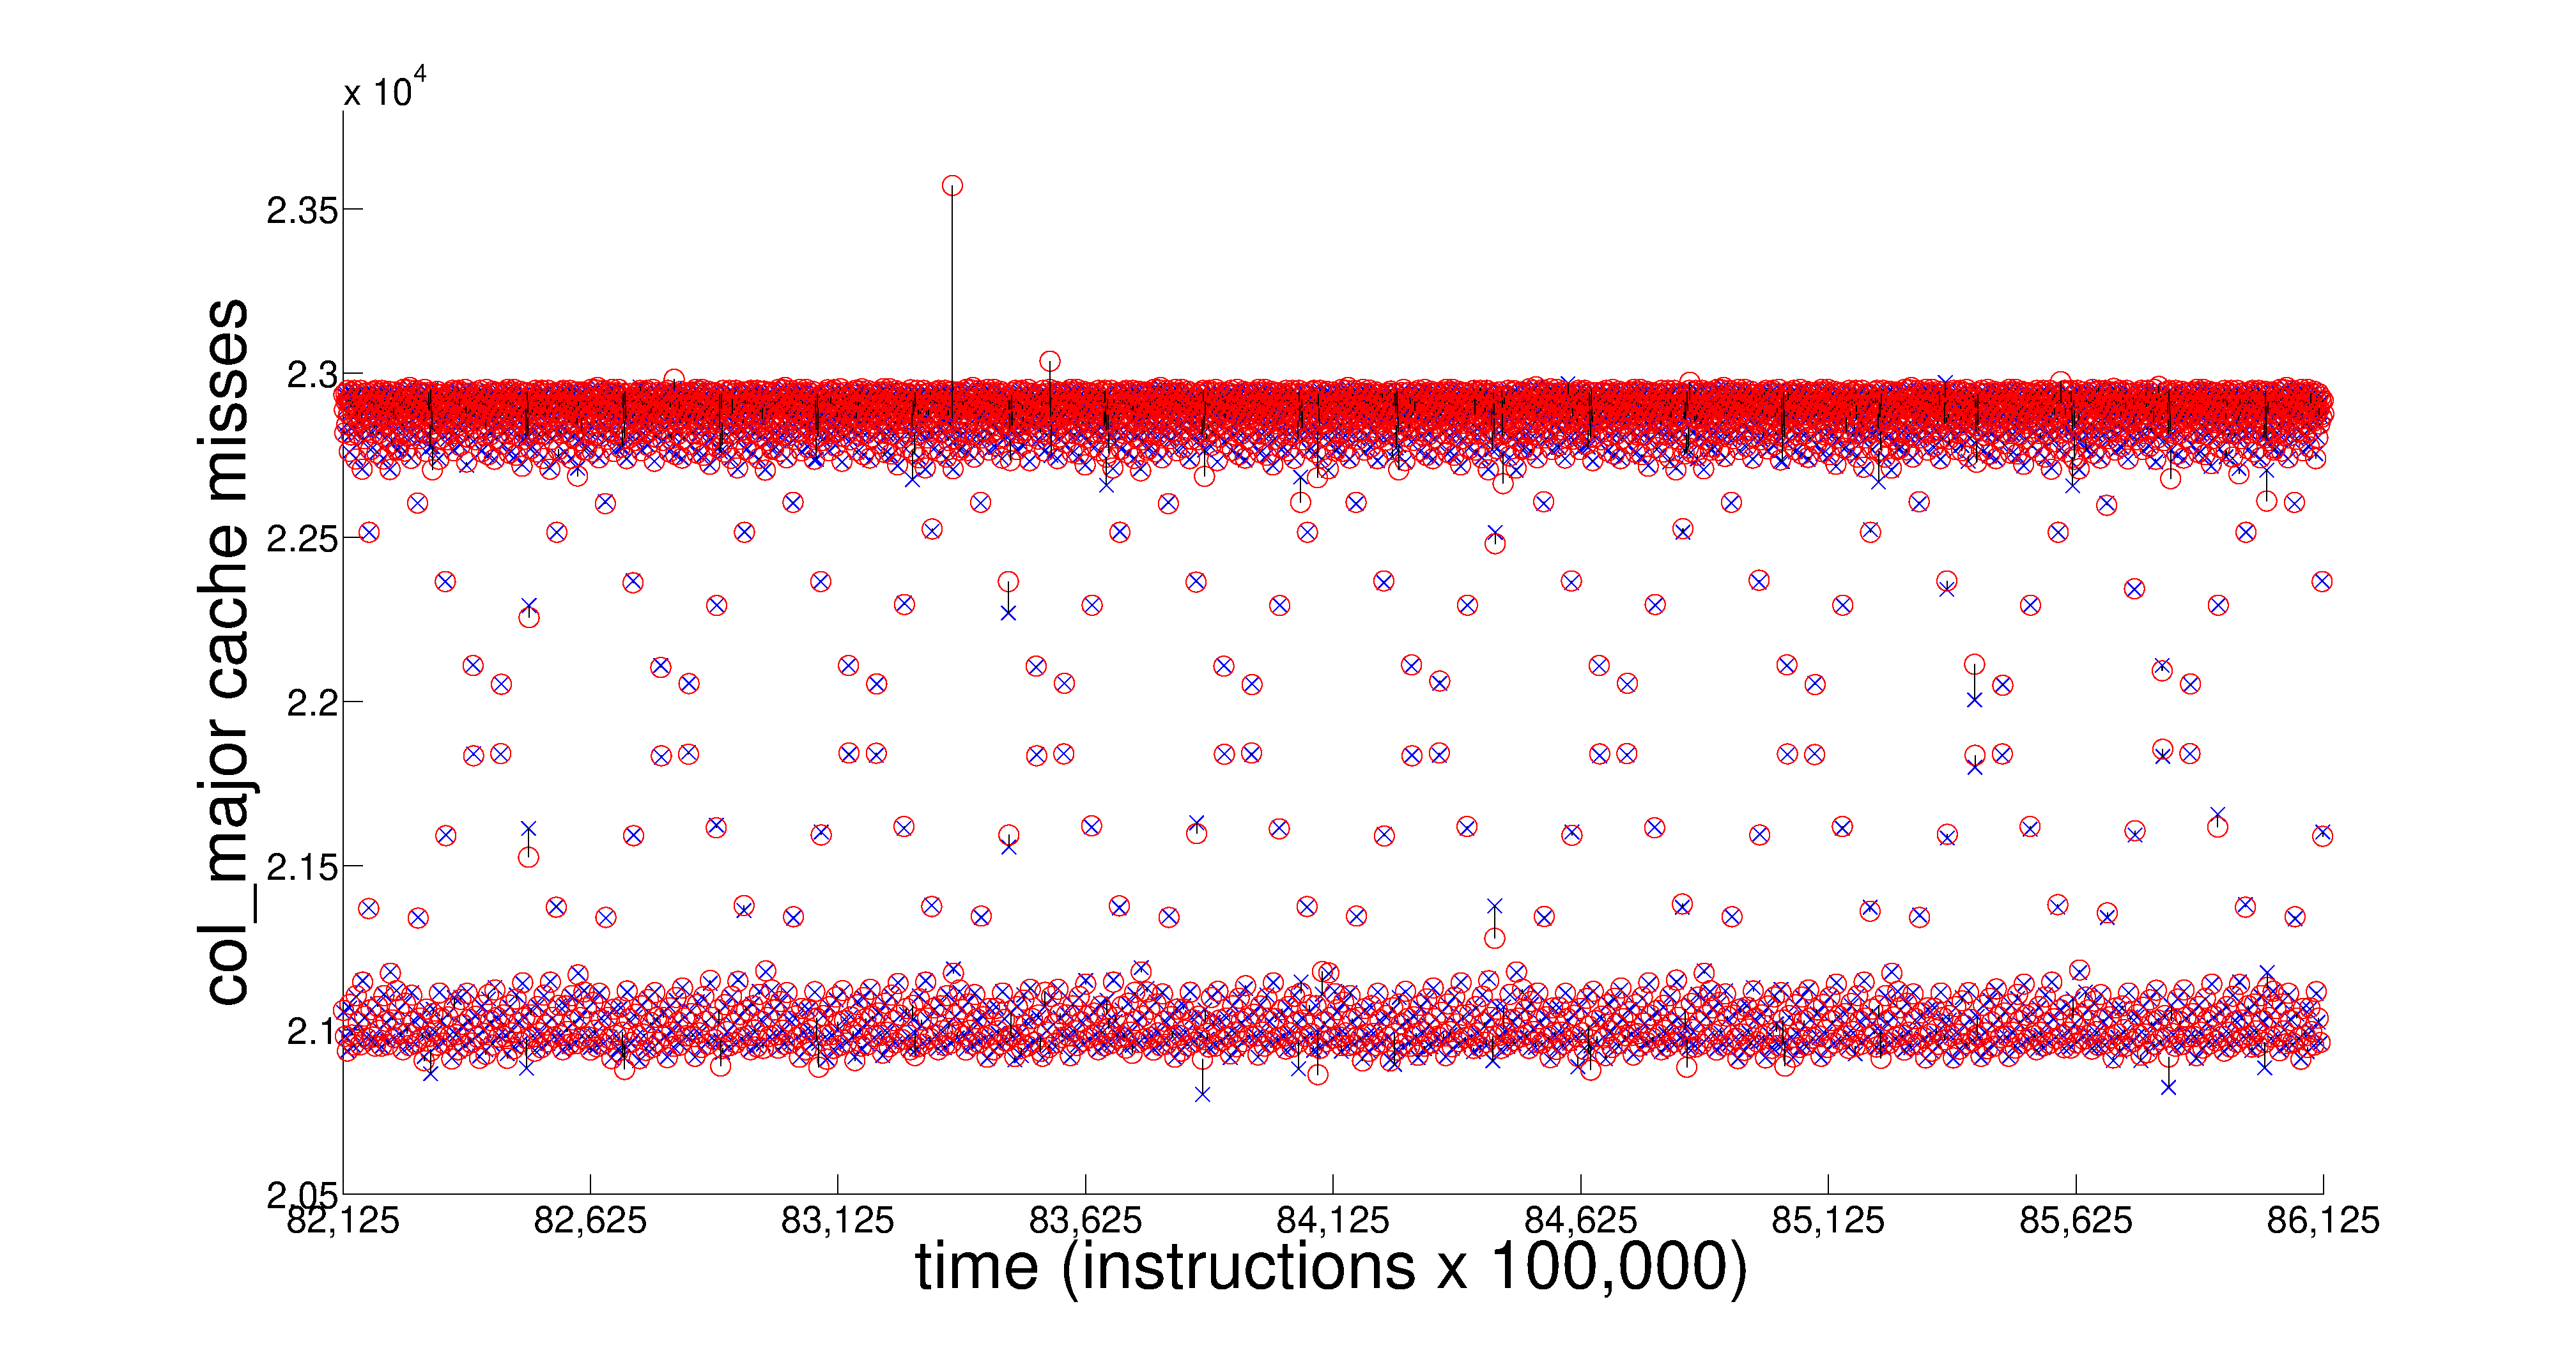
\includegraphics[width=0.5\textwidth]{figs/colCachePredTS}
    \caption{A forecast of the last 4,000 points of the signal in
      Figure~\ref{fig:cache} using an LMA-based strategy on the
      embedding in Figure~\ref{fig:embedding}.  Red circles and blue
      $\times$s are the true and predicted values, respectively;
      vertical bars show where these values differ. }
\label{fig:cachePredTS}
\end{figure}
%
On the other hand, if we use the same approach to forecast the
processor load\footnote{Instructions per cycle, or IPC} of the {\tt
  482.sphinx3} program from the SPEC cpu2006 benchmark suite, running
on an Intel i7\textsuperscript{\textregistered}-based machine, the
prediction is far less accurate; see Figure~\ref{fig:predsphinx}.
%
\begin{figure}[htbp]
  \centering
    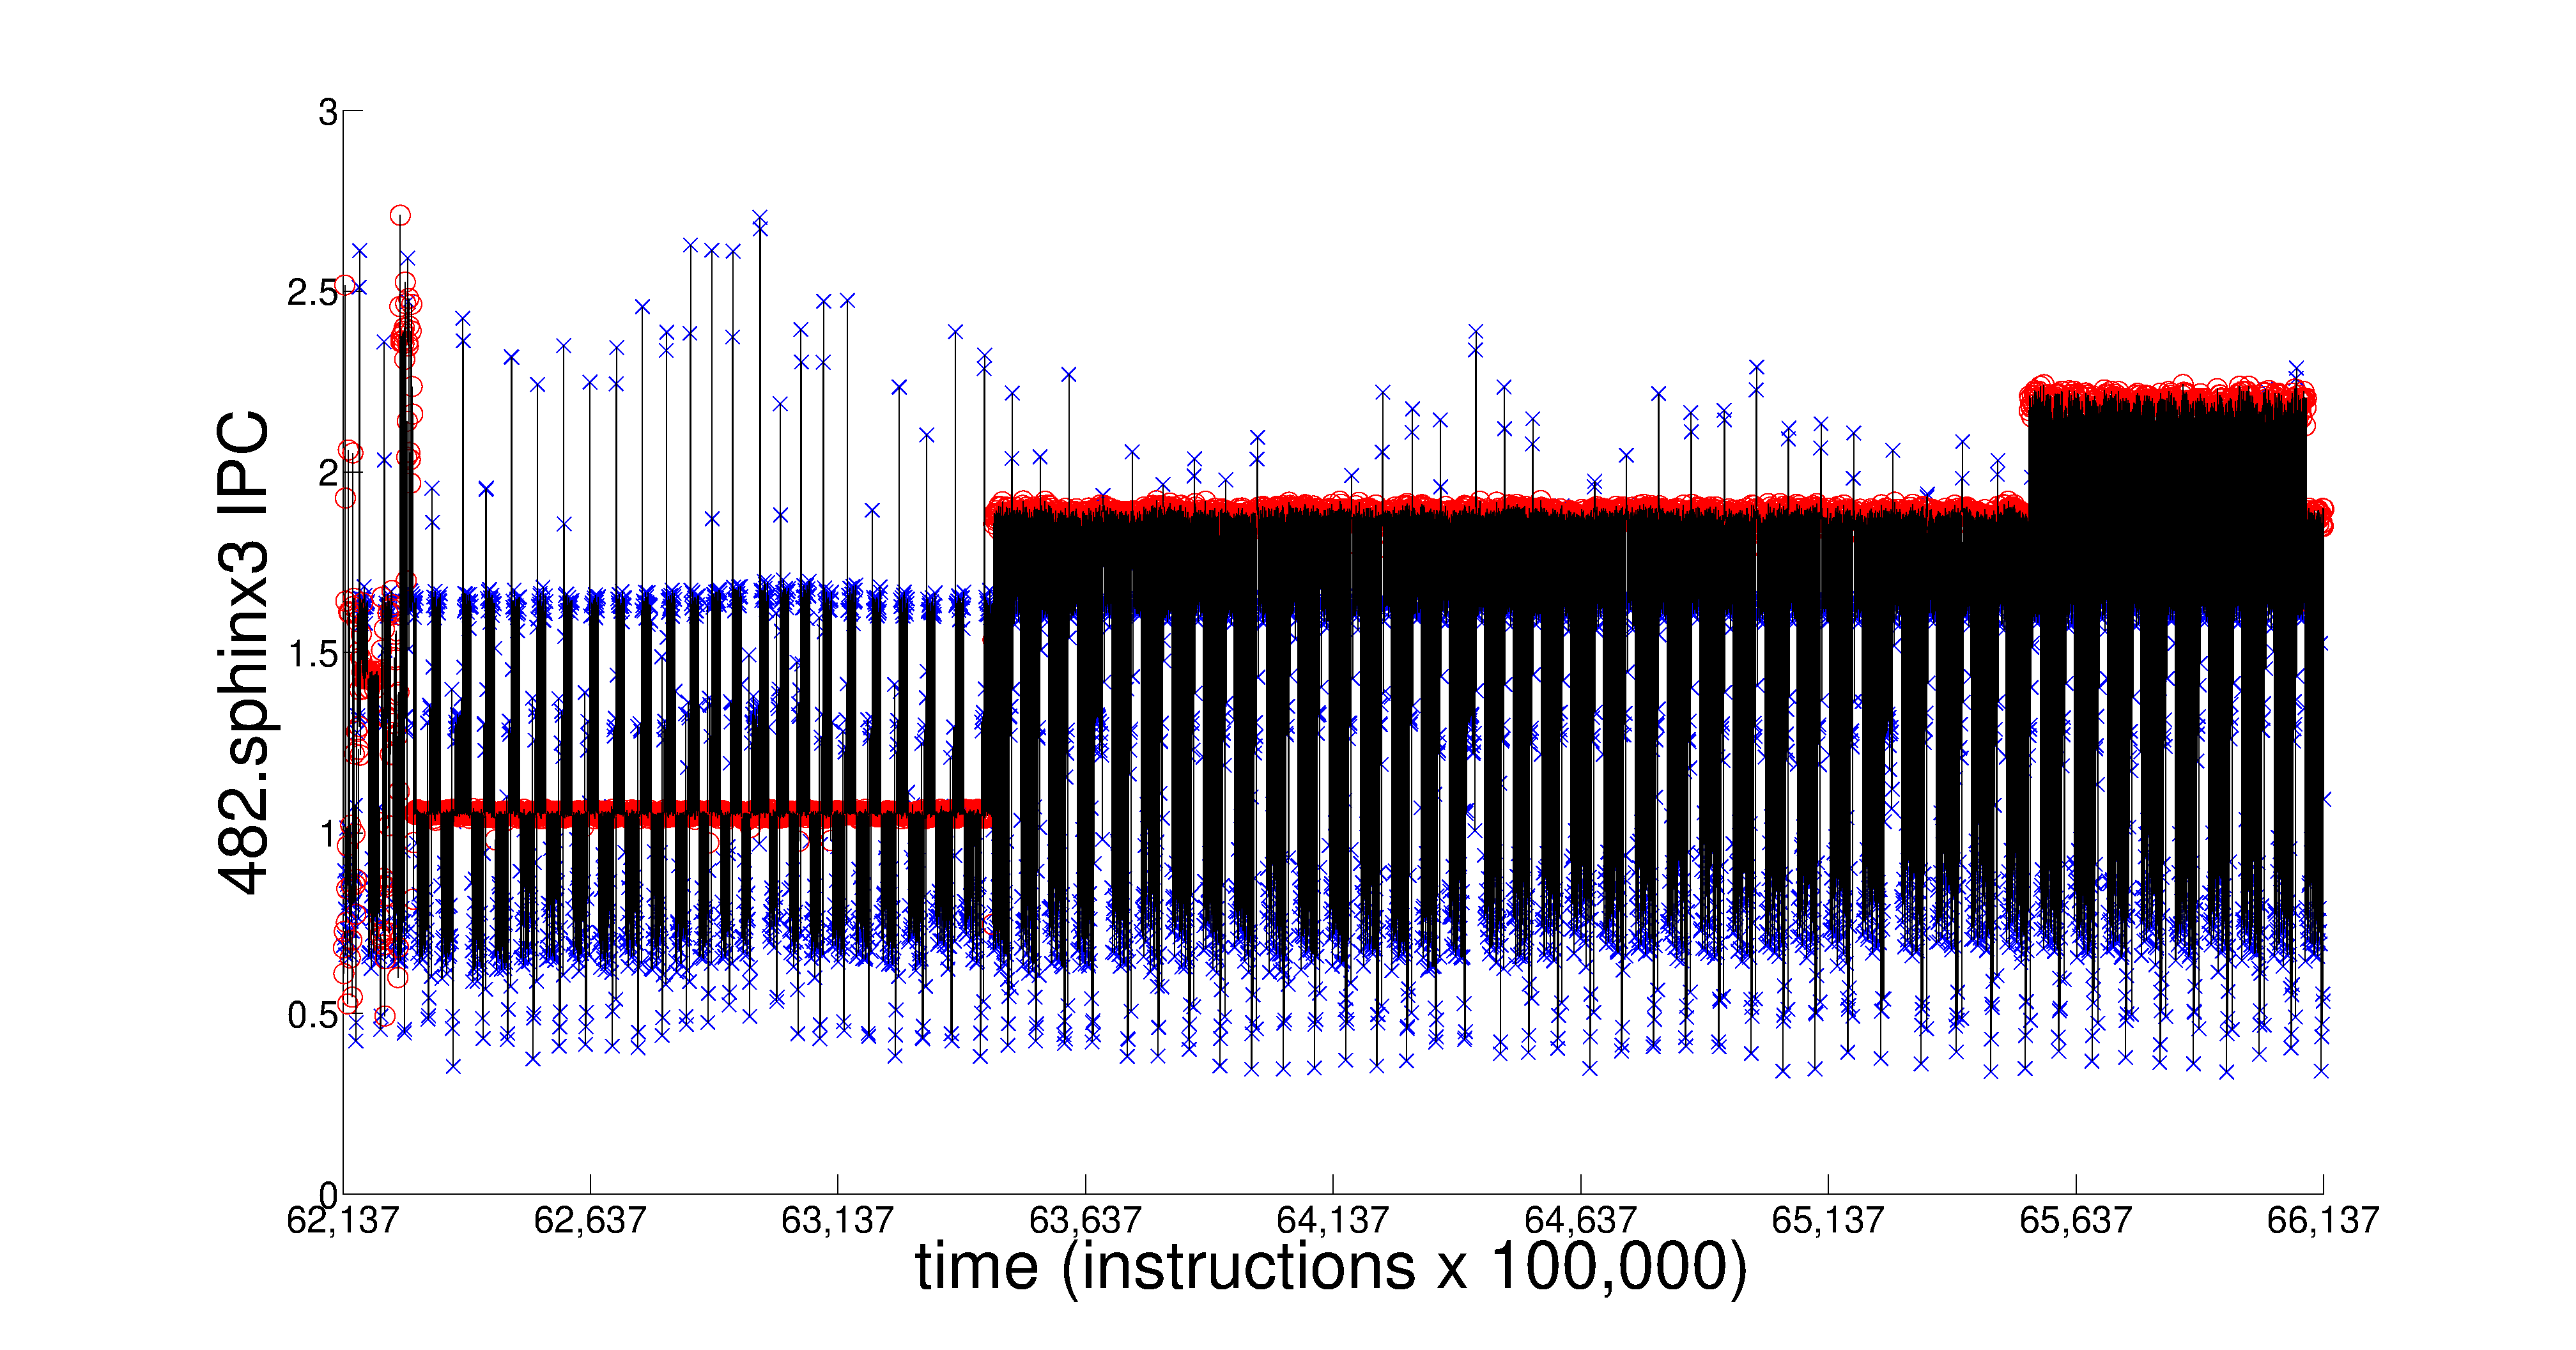
\includegraphics[width=0.5\textwidth]{figs/sphinxPredicTS}
     \caption{An LMA-based forecast of the last 4,000 points of a
       processor-load performance trace from the {\tt 482.sphinx3}
       benchmark.  Red circles and blue $\times$s are the true and
       predicted values, respectively; vertical bars show where these
       values differ.}
\label{fig:predsphinx}
\end{figure}

Table~\ref{tab:PredError} presents detailed results about the
prediction accuracy of this algorithm on four different examples: the
{\tt col\_major} and {\tt 482.sphinx3} programs in
Figures~\ref{fig:cachePredTS} and~\ref{fig:predsphinx}, as well as
another simple microkernel that initializes the same matrix as {\tt
  col\_major}, but in row-major order, and another complex program
({\tt 403.gcc}) from the SPEC cpu2006 benchmark suite.  Both
microkernels were run on the Intel Core
Duo\textsuperscript{\textregistered} machine; both SPEC benchmarks
were run on the Intel i7\textsuperscript{\textregistered} machine.  We
calculated a figure of merit for each prediction as follows.  We held
back the last $k$ elements\footnote{Several different prediction
  horizons were analyzed in our experiment; the results reported in
  this paper are for $k$=4000} of the $N$ points in each measured time
series, built the forecast model by embedding the first $N-k$ points,
used that embedding and the LMA method to predict the next $k$ points,
then computed the Root Mean Squared Error (RMSE) between the true and
predicted signals:
$$RMSE = \sqrt{\frac{\sum_{i=1}^k(c_i-\hat{p_i})^2}{k}}$$
%
To compare the success of predictions across signals with different
units, we normalized RMSE as follows:
$$nRMSE = \frac{RMSE}{X_{max,obs}-X_{min,obs}}$$
%
% The smaller the nRMSE, obviously, the more accurate the prediction.

  \begin{table}[htbp]
   % increase table row spacing, adjust to taste
   \renewcommand{\arraystretch}{1.3}
   \caption{Normalized root mean squared error (nRMSE) of 4000-point
     predictions of memory \& processor performance from different
     programs.}
   \label{tab:PredError}
   \centering
   % Some packages, such as MDW tools, offer better commands for making tables
   % than the plain LaTeX2e tabular which is used here.
%   \begin{tabular}{|c|c|c|c|c|c|}
%     \hline
%      & cache misses NRMSE & IPC NRMSE \\
%     \hline
%     \tt{row\_major}  & 0.0102  & 0.0095 \\
%          \hline
%     \tt{col\_major}  &0.0055& 0.0071 \\
%     \hline
%     \tt{403.gcc}  & 0.0865& 0.1805 \\
%          \hline
%     \tt{482.sphinx3} & 0.1142& 0.2946 \\
%      \hline
%   \end{tabular}
% \end{table}
   \begin{tabular}{|c|c|c|c|c|c|}
     \hline
      & cache miss rate & instrs per cycle \\
     \hline
     \tt{row\_major}  & 0.0324  & 0.0778 \\
          \hline
     \tt{col\_major}  &0.0080& 0.0161 \\
     \hline
     \tt{403.gcc}  & 0.1416& 0.2033 \\
          \hline
     \tt{482.sphinx3} & 0.2032& 0.3670 \\
      \hline
   \end{tabular}
 \end{table}

The results in Table~\ref{tab:PredError} show a clear distinction
between the two microkernels, whose future behavior can be
predicted effectively using this simple deterministic modeling
strategy, and the more-complex SPEC benchmarks, for which this
prediction strategy does not work nearly as well.
% Removed for space
% For both processor load (IPC) and memory usage (cache-miss rate),
% forecasts for {\tt 482.sphinx3} and {\tt 403.gcc} are much worse than
% for \verb|col_major| or \verb|row_major|.
%
This begs the question: If these traces all come from deterministic
systems---computers---then why are they not equally predictable?  Our
conjecture is that the sheer complexity of the dynamics of the SPEC
benchmarks running on the Intel i7\textsuperscript{\textregistered}
machine make them effectively impossible to predict.

%% [[If space: Add a segue sentence: next section uses permutation
%% entropy to explore that conjecture.]]

\section{Measuring Complexity}\label{sec:meaComplex}

For the purposes of this paper, one can view entropy as a measure of complexity
and predictability in a time series.  A high-entropy time series is almost
completely unpredictable---and conversely.  This can be made more rigorous:
Pesin's relation \cite{pesin77} states that in chaotic dynamical systems, the
Shannon entropy rate is equal to the sum of the positive Lyapunov exponents,
$\lambda_i$. The Lyapunov exponents directly quantify the rate at which nearby
states of the system will diverge with time: $\left| \Delta x(t) \right| \approx
e^{\lambda t} \left| \Delta x(0) \right|$.  The faster the divergence, the more
difficult prediction becomes.

Utilizing entropy as a measure of temporal complexity is by no means a new idea
\cite{Shannon1951, mantegna1994linguistic}.  Its effective usage requires
categorical data: $x_t \in \mathcal{S}$ for some finite or countably infinite
\emph{alphabet} $\mathcal{S}$, whereas data taken from real-world systems is
effectively real-valued.  To get around this, one must discretize the data---
typically achieved by binning.  Unfortunately, this is rarely a good solution to
the problem, as the binning of the values introduces an additional dynamic on
top of the intrinsic dynamics whose entropy is desired.  The field of symbolic
dynamics studies how to discretize a time series in such a way that the
intrinsic behavior is not perverted, but these methods are fragile in the face
of noise and require further understanding of the underlying system, which
defeats the purpose of measuring the entropy in the first place.

Bandt and Pompe introduced the \emph{permutation entropy} (PE) as a ``natural
complexity measure for time series" \cite{bandt2002per}.  Permutation entropy
employs a method of discretizing real-valued time series that follows the
intrinsic behavior of the system under examination.  Rather than looking at the
statistics of sequences of values, as is done when computing the Shannon
entropy, permutation entropy looks at the statistics of the \emph{orderings} of
sequences of values using ordinal analysis. Ordinal analysis of a time series is
the process of mapping successive time-ordered elements of a time series to
their value-ordered permutation of the same size.  By way of example, if $(x_1,
x_2, x_3) = (9, 1, 7)$ then its \emph{ordinal pattern}, $\phi(x_1, x_2, x_3)$,
is $231$ since $x_2 \leq x_3 \leq x_1$.  This method has many features; among
other things, it is generally robust to observational noise and requires no
knowledge of the underlying mechanisms.

\begin{mydef}[Permutation Entropy]

  Given a time series $\{x_t\}_{t = 1,\dots,T}$. Define $\mathcal{S}_n$ as all
  $n!$ permutations $\pi$ of order $n$. For each $\pi \in \mathcal{S}_n$ we
  determine the relative frequency of that permutation occurring in $\{x_t\}_{t
  = 1,\dots,T}$:
  \begin{align*}
    p(\pi) = \frac{\left|\{t|t \leq T-n,\phi(x_{t+1},\dots,x_{t+n}) = \pi\}\right|}{T-n+1}
  \end{align*}
  Where $|\cdot|$ is set cardinality. The \emph{permutation entropy} of order $n
  \ge 2$ is defined as
  \begin{align*}
  H(n) = - \sum_{\pi \in \mathcal{S}_n} p(\pi) \log_2 p(\pi)
  \end{align*}

\end{mydef}

Notice that $0\le H(n) \le \log_2(n!)$ \cite{bandt2002per}.  With this in mind,
it is common in the literature to normalize permutation entropy as follows:
$\frac{H(n)}{\log_2(n!)}$.  With this convention, ``low'' entropy is close to 0
and ``high'' entropy is close to 1. Finally, it should be noted that the
permutation entropy has been shown to be identical to the Shannon entropy for
many large classes of systems \cite{amigo2012permutation}.

Here we will be utilizing a variation of the permutation entropy, the
\emph{weighted permutation entropy} (WPE)~\cite{fadlallah2013}. The weighted
permutation entropy attempts to correct for observational noise which is larger
than some trends in the data, but smaller than the larger scale features --- for
example, a signal that switches between two fixed points with noise about those
fixed points. The weighted permutation entropy would be dominated by the
switching rather than by the stochastic fluctuation. To accomplish this, the
\emph{weight} of a permutation is taken into account:
\begin{align*}
  w(x_{t+1:t+n}) = \frac{1}{n}
                 \sum_{x_i \in \{x_{t+1:t+n}\}}
                 \left( x_i - \bar{x}_{t+1:t+n} \right)^2
\end{align*}
where $x_{t+1:t+n}$ is a sequence of values $x_{t+1}, \ldots, x_{t+n}$, and
$\bar{x}_{t+1:t+n}$ is the arithmetic mean of those values.

The weighted probability of a permutation is then:
\begin{align*}
  p_w(\pi) = \frac{\displaystyle \sum_{t \le T - n} w(x_{t+1:t+n}) \cdot \delta(\phi(x_{t:t+n}), \pi) }{\displaystyle \sum_{t \le T - n} w(x_{t+1:t+n})}
\end{align*}
where $\delta(x, y)$ is 1 if $x = y$ and 0 otherwise. Effectively, this weighted
probability enhances permutations involved in ``large'' features and demotes
permutations which are small in amplitude relative to the features of the time
series. The weighted permutation entropy is then:
\begin{align*}
  H_w(n) = - \sum_{\pi \in \mathcal{S}_n} p_w(\pi) \log_2 p_w(\pi),
\end{align*}
which can also be normalized by dividing by $\log_2(n!)$, and will be in all the
results of this paper.

In practice, calculating permutation entropy and weighted permutation entropy
involves choosing a good value for the word length $n$. The primary
consideration is that the value be large enough that forbidden ordinals are
discovered, yet small enough that reasonable statistics over the ordinals are
gathered: e.g.:
\begin{align*}
  n = \operatornamewithlimits{argmax}_\ell \{ T \gtrapprox 100 \ell! \},
\end{align*}
assuming an average of 100 counts per ordinal is sufficient. In the literature,
$3 \le n \le 6$ is a standard choice --- generally without any formal
justification. In theory, the permutation entropy should reach an asymptote with
increasing $n$, but that requires an arbitrarily long time series. In practice,
what one should do is calculate the \emph{persistent} permutation entropy by
increasing $n$ until the result converges, but data length issues can intrude
before that convergence is reached.

The weighted permutation entropy for the {\tt SVD} program is given in
Fig.~\ref{fig:wwpe}. To generate this image a window of 5,000 values slid over
the time series. Within each of those windows, the statistics over words of
length 4 are computed and the WPE is calculated. The gray bands denote regions
where the 5,000 value window overlapped visually-distinct regimes. It can be
seen that the behaviors of the weighted permutation entropy vary between
regimes.

\begin{figure}[htbp]
  \centering
  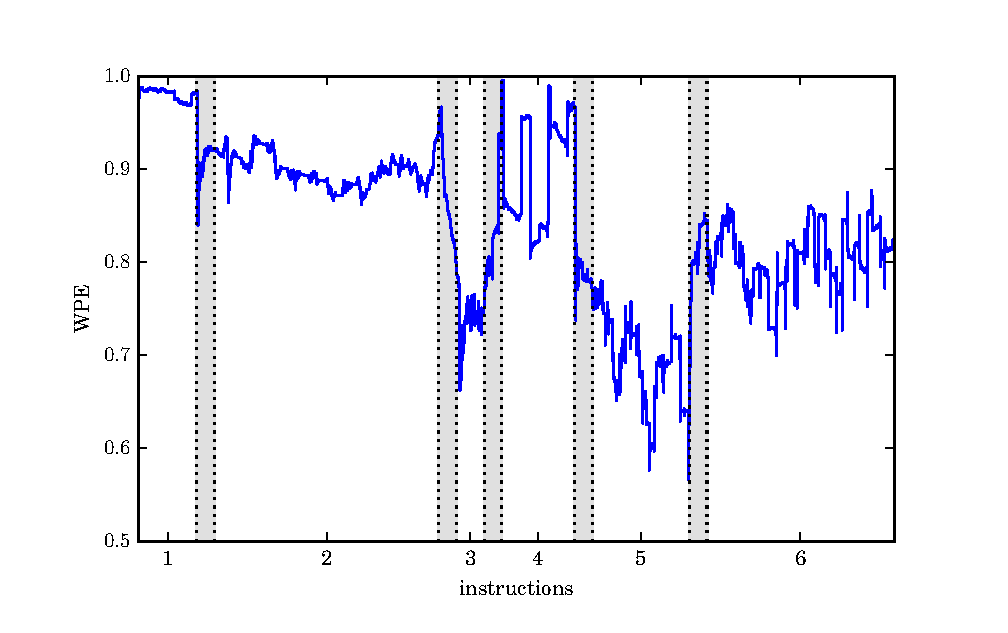
\includegraphics[width=1.0\textwidth]{figs/SVD_wwpe}
  \caption{The weighted permutation entropy of one run of SVD. The gray bands
    are regions where the window overlaps regimes. The window size used is
    $5,000 \times 100,000$ instructions and the word length is $4$.}
  \label{fig:wwpe}
\end{figure}


% Table~\ref{tab:pe} shows the permutation entropy results for the
% examples considered in this paper, with the nRMSPE prediction
% accuracies from the previous section included alongside for easy
% comparison.
%
% \begin{table}[htbp]
%   % increase table row spacing, adjust to taste
%   \renewcommand{\arraystretch}{1.3}
%   \caption{TCM NRMSE and PE NORMS}
%   \label{tab:table_example}
%   \centering
   % Some packages, such as MDW tools, offer better commands for making tables
   % than the plain LaTeX2e tabular which is used here.
%   \begin{tabular}{|c|c|c|c|c|c|}
%     \hline
%     TCM & NRMSE & $m=3$  &$m=4$&$m=5$&$m=6$\\
%     \hline
%     \tt{row\_major} & 0.0102 & 0.7900  &0.6751&0.5458&0.4491\\
%     \hline
%     \tt{col\_major} & 0.0055 & 0.6411  &0.5029&0.4515&0.3955 \\
%     \hline
%     \tt{403.gcc} & 0.0865 & 0.9954  &0.9916&0.9880&0.9835\\
%     \hline
%     \tt{482.sphinx3} & 0.1142 & 0.9958  &0.9913&0.9866&0.9802 \\
%      \hline
%   \end{tabular}
% \end{table}
%
%%  \begin{table}[htbp]
%%   % increase table row spacing, adjust to taste
%%   %\renewcommand{\arraystretch}{1.3}
%%   \caption{Cache-miss rate performance traces: prediction error
%%     (nRMSPE) and permutation entropy}
%%   \label{tab:TCMpe}
%%   \centering
%%   % Some packages, such as MDW tools, offer better commands for making tables
%%   % than the plain LaTeX2e tabular which is used here.
%%   \begin{tabular}{|c|c|c|c|c|c|}
%%     \hline
%%      & nRMSE   &$n=4$&$n=5$&$n=6$\\
%%     \hline
%%     \tt{row\_major}  & 0.0324  &0.6751&0.5458&0.4491\\
%%     \hline
%%     \tt{col\_major}  & 0.0080  &0.5029&0.4515&0.3955 \\
%%     \hline
%%     \tt{403.gcc}  & 0.1416  &0.9916&0.9880&0.9835\\
%%     \hline
%%     \tt{482.sphinx3}  & 0.2032  &0.9913&0.9866&0.9802 \\
%%      \hline
%%   \end{tabular}
%% \end{table}
%
% \begin{table}[htbp]
%   % increase table row spacing, adjust to taste
%   \renewcommand{\arraystretch}{1.3}
%   \caption{IPC NRMSE and PE NORMS}
%   \label{tab:table_example}
%   \centering
%   % Some packages, such as MDW tools, offer better commands for making tables
%   % than the plain LaTeX2e tabular which is used here.
%   \begin{tabular}{|c|c|c|c|c|c|}
%     \hline
%     ipc & NRMSE & $n=3$  &$n=4$&$n=5$&$n=6$\\
%     \hline
%      \tt{row\_major} & 0.0095 & 0.9912  &0.9723&0.9354&0.8876\\
%     \hline
%      \tt{col\_major} & 0.0071 & 0.9428  &0.8356&0.7601&0.6880\\
%     \hline
%     \tt{403.gcc} & 0.1805 & 0.9918  &0.9862&0.9814&0.9764\\
%     \hline
%     \tt{482.sphinx3} & 0.2946 & 0.9978  &0.9951&0.9914&0.9849 \\
%      \hline
%   \end{tabular}
% \end{table}
%
%%  \begin{table}[htbp]
%%   % increase table row spacing, adjust to taste
%%   %\renewcommand{\arraystretch}{1.1}
%%   \caption{Processor load performance traces: prediction error
%%     (nRMSPE) and permutation entropy}
%%   \label{tab:IPCpe}
%%   \centering
%%   % Some packages, such as MDW tools, offer better commands for making tables
%%   % than the plain LaTeX2e tabular which is used here.
%%   \begin{tabular}{|c|c|c|c|c|}
%%     \hline
%%      & nRMSPE   &$n=4$&$n=5$&$n=6$\\
%%     \hline
%%      \tt{row\_major} & 0.0778  &0.9723&0.9354&0.8876\\
%%     \hline
%%      \tt{col\_major} & 0.0161   &0.8356&0.7601&0.6880\\
%%     \hline
%%     \tt{403.gcc} & 0.2033   &0.9862&0.9814&0.9764\\
%%     \hline
%%     \tt{482.sphinx3} & 0.3670 & 0.9951&0.9914&0.9849 \\
%%      \hline
%%   \end{tabular}
%% \end{table}
%
 %  \begin{table}[htbp]
 %   \caption{Prediction error (in nRMSPE) and permutation entropy (for
 %     different wordlengths $n$}
 %   \label{tab:pe}
 %   \centering
 %   \begin{tabular}{|c|c|c|c|c|c|}
 %     \hline
 %      {\bf cache misses} & error   &$n=4$&$n=5$&$n=6$\\
 %     \hline
 %     \tt{row\_major}  & 0.0324  &0.6751&0.5458&0.4491\\
 %     \hline
 %     \tt{col\_major}  & 0.0080  &0.5029&0.4515&0.3955 \\
 %     \hline
 %     \tt{403.gcc}  & 0.1416  &0.9916&0.9880&0.9835\\
 %     \hline
 %     \tt{482.sphinx3}  & 0.2032  &0.9913&0.9866&0.9802 \\
 %      \hline
 %      \hline
 %      {\bf insts per cyc} & error   &$n=4$&$n=5$&$n=6$\\
 %     \hline
 %      \tt{row\_major} & 0.0778  &0.9723&0.9354&0.8876\\
 %     \hline
 %      \tt{col\_major} & 0.0161   &0.8356&0.7601&0.6880\\
 %     \hline
 %     \tt{403.gcc} & 0.2033   &0.9862&0.9814&0.9764\\
 %     \hline
 %     \tt{482.sphinx3} & 0.3670 & 0.9951&0.9914&0.9849 \\
 %      \hline
 %   \end{tabular}
 % \end{table}

 \section{Results} % (fold)
 \label{sec:results}



First paragraph: WPE is a good measure of predictability.  Figure:
best athlete MASE vs. its WPE.

The relationship between prediction accuracy and the weighted permutation
entropy (WPE) is much as we conjectured: performance traces with high WPE are
indeed harder to predict using the forecasting models described in the prior
section. Figure~\ref{fig:pred_vs_ent} demonstrates this primary finding, with
the exception of one outlier whose behavior we can explain. Furthermore, we find
that the relationship between the two is roughly linear. The single outlier,
{\tt SVD} regime 1, does not fit the trend due to a weakness in the WPE: namely
that in the absence of any large features, as all the other regimes have, the
WPE effectively falls back to the standard PE for which the noisy behavior
drives toward 1.0.


The structure being picked up on by WPE may be linear or nonlinear. When you have a low WPE and a high ARIMA it could be that the structure WPE is picking up is simply nonlinear structure that LMA can handle but ARIMA cannot. So while the ARIMA prediction look realy bad there is plenty of structure present as suggested by WPE and taken advantage of by LMA but since it is nonlinear ARIMA can't take it into account and does bad.


\begin{figure}[htbp]
  \centering
  \includegraphics[width=1.0\textwidth]{figs/prediction_vs_entropy}
  \caption{The best MASE among all runs and prediction methods vs weighted
  permutation entropy. For each of these, the word length used is $6$. The
  dashed line is a least-squares linear fit of all the points except for {\tt
  SVD$_1$} which we have excluded for reasons explained in the text.}
  \label{fig:pred_vs_ent}
\end{figure}

Second paragraph: full results.  Image: MASE vs. WPE for both LMA \&
ARIMA.  Points to make: (1) clusters are distributed differently (2)
clusters are shaped differently---tight or not (3) clusters move
differently between LMA and ARIMA (4) finally, the diagonal line is
important.  If you're below it, you could do better.







\begin{figure}[htbp]
  \centering
  \includegraphics[width=1.0\textwidth]{figs/prediction_vs_entropy}
  \caption{The best MASE among all runs and prediction methods vs weighted
  permutation entropy. For each of these, the word length used is $6$. The
  dashed line is a least-squares linear fit of all the points except for {\tt
  SVD$_1$} which we have excluded for reasons explained in the text.}
  \label{fig:pred_vs_ent}
\end{figure}

In Figures~\ref{fig:lma_pred_vs_ent} and \ref{fig:arima_pred_vs_ent} we directly
compare the performance of the LMA and ARIMA prediction methods (respectively)
to the value of the weighted permutation entropy for all runs of each program
under consideration. The LMA MASE values are largely similar to those of the
best predictions, primarily because LMA often performed superior to ARIMA and
the naive method. On the other hand, the ARIMA MASE values are largely
uncorrelated with WPE values. This however does not contradict our hypothesis,
it just means that ARIMA is ill-suited for the time series under investigation.
To see this more clearly, consider Figure~\ref{fig:lma_vs_arima}. Since larger
MASE values constitute worse predictions, ARIMA performed worse than LMA in all
traces except {\tt SVD$_1$}.

\begin{figure}[htbp]
  \centering
  \begin{subfigure}{0.5\textwidth}
    \includegraphics[width=1.0\textwidth]{figs/LMA_prediction_vs_entropy}
    \caption{The MASE of LMA vs weighted permutation entropy. For each of these,
    the word length used is $6$.}
    \label{fig:lma_pred_vs_ent}
  \end{subfigure}%
  \begin{subfigure}{0.5\textwidth}
    \includegraphics[width=1.0\textwidth]{figs/ARIMA_prediction_vs_entropy}
    \caption{The MASE of ARIMA vs weighted permutation entropy. For each of
    these, the word length used is $6$.}
    \label{fig:arima_pred_vs_ent}
  \end{subfigure}
  \begin{subfigure}{0.5\textwidth}
    \includegraphics[width=1.0\textwidth]{figs/LMA_vs_ARIMA}
    \caption{The MASE values for LMA against ARIMA. The dashed line is the
    identity, delineating the traces for which either LMA or ARIMA performed
    better. All traces except those from {\tt SVD$_1$} lie above the line,
    indicating that LMA is better suited prediction method for the computer
    traces considered.}
    \label{fig:lma_vs_arima}
  \end{subfigure}
\end{figure}

 % section results (end)

% In Table~\ref{tab:TCMpe} \& \ref{tab:IPCpe} the behavior of the PEs as
% they limit to their asymptotic values is observed. A feature of note
% is that some of the signals drop off and some do not.  For example at
% $m=4$ {\tt col\_major} is at 0.8356, a fairly high entropy, however as
% $m$ is increased to 6 the PE plummets to 0.6880: a value consistent
% with a chaotic time series. Notice this also corresponds to a very low
% nRMSE. In contrast, consider the permutation entropy of the processor
% load of {\tt 482.sphinx3}: with $m=4$ it is 0.9951 and only drops to
% 0.9849 at $m=6$. This is consistent with the signal also having the
% highest nRMSE.

\section{ Conclusions \& Future Work}\label{sec:conc}

The results presented here suggest that permutation entropy---a ordinal
calculation of forward information transfer in a time series---is an effective
metric for predictability of computer performance traces. Experimentally, traces
with a persistent PE $\gtrapprox 0.97$ have a natural level of complexity that
may overshadow the inherent determinism in the system dynamics, whereas traces
with PE $\lessapprox 0.7$ seem to be highly predictable (viz., at least an order
of magnitude improvement in nRMSPE).Further, the persistent WPE values of 0.5--
0.6 for the {\tt col\_major} trace are consistent with dynamical chaos, further
corroborating the results of~\cite{mytkowicz09}.

If information is the limit, then gathering and using more information is an
obvious next step.  There is an equally obvious tension here between data length
and prediction speed: a forecast that requires half a second to compute is not
useful for the purposes of real-time control of a computer system with a MHz
clock rate.  Another alternative is to sample several system variables
simultaneously and build multivariate delay-coordinate embeddings.  Existing
approaches to that are computationally prohibitive
\cite{cao-multivariate-embedding}.  We are working on alternative
methods that sidestep that complexity.

%%This use of permutaiotn entropy is a useful application of information
%%theory to computer performance modeling because it gives you a simple
%%and fast way to decide whether building a model and trying to forecast
%%the future is worthwhile or if guessing the mean is just as effective.
%%End with a sentence tying back to power management and world peace.


%\begin{it}
%Summarize the results.

%Paragraphs on the issues that come up, including one about the "amount
%of info" one: if one could sample more variables, for instance, one
%might be able to do a better job of predicting more-complex traces.
%Segue to some handwaving about multivariable LMA models; tie this back
%to the "computers are NLD systems" stuff in the intro.  This is a real
%challenge; current approaches to this modelling problem have the major
%issue of taking way too long to build.  And that's a big issue if
%you're trying not just to classify, but to predict.  In a system that
%runs at MHz speeds, a prediction that takes milliseconds to compute is
%not useful.
%\end{it}




%[[Joshua: It may be interesting to look at the PE as a function of
%prediction horizon. It is known to me that certain start and end
%locations in the prediction strategy result in different prediction
%accuracy. Is it the case that when the algorithm tanks it is also the
%case that PE of the **TEST**(the 10\% we cut off )is high? This may
%be a great way to illustrate the concept if it works... OR maybe do
%complexity of forward path in embedding space?]]  some notes about
%this looking at row Cache 1000 very good RMSPE 21.4167 m = 3 4 5 6
%1.4192 2.1286 2.5942 2.9230 row Cache 2000 very good RMSPE 19.0990 m
%= 3 4 5 6 1.4145 2.1305 2.5825 2.9095 so even better row Cache 2010
%RMSPE 19.9716 m = 3 4 5 6 1.4149 2.1311 2.5830 2.9096 row Cache 1990
%RMSPE 19.1465 So prediction Horizons ranked in order of best RMSPE
%RMSPE L 3 4 5 6 1st 19.0990 2000 1.4145 2.1305 2.5825 2.9095 2nd
%19.1465 1990 1.4151 2.1293 2.5803 2.9067 3rd 19.9716 2010 1.4149
%2.1311 2.5830 2.9096 3rd 21.4167 1000 1.4192 2.1286 2.5942 2.9230
%ipcgcc m = 3 pe = 1.7770 penorm = 0.9918 m= 4 pe = 3.1341 penorm =
%0.9862 m = 5 pe = 4.6985 penorm = 0.9814 m=6 pe = 6.4242 penorm =
%0.9764 m=7 pe = 8.2450 penorm = 0.9671 >> [pe penorm] =
%permCalc(gcc100TCM,5,1) pe = 4.7299 penorm = 0.9880 >> [pe penorm] =
%permCalc(gcc100TCM,6,1) pe = 6.4707 penorm = 0.9835





\section{New Figures and Tables}

Possible new error measure

$$q_t = \frac{e_t}{\frac{1}{n-1}\sum^n_{i=2}|Y_i-Y_{i-1}|}$$

$$MASE = mean(|q_t|)$$

Helpful to remember that $F_i = Y_{i-1}$ for random walk prediction

``When $MASE<1$, the proposed method gives, on average, smaller errors than the one-step errors from the na\"ive method. If multi-step forecasts are being computed, it is possible to scale by the in- sample MAE[[Mean Absolute Error(mean($|e_t|$)]] computed from multi-step na\"i�ve forecasts."

``The errors have been scaled by the one-step in- sample forecast errors from the na\"ive method, and then averaged across all series. So a value of 2 indicates that the out-of-sample forecast errors are, on average, about twice as large as the in-sample one-step forecast errors from the na\"ive method. Because the scaling is based on one-step forecasts, the scaled errors for multi-step forecasts are typically larger than one. "

We use this error measure with $n$ at the start of the predicted chunk.

\begin{table}[htdp]
\caption{ Embedding Parameters for reference if needed. }
\begin{center}
\begin{tabular}{|c|c|c|}
\hline
&$\tau$ & $m$ \\
\hline
gcc & 10& 13\\
col\_major  &2&12\\
SVD\_Full &  10  &  12 \\
SVD\_IPC\_Regime1 & 5 &14  \\
SVD\_IPC\_Regime2 & 10   &12  \\
SVD\_IPC\_Regime3 & 2   &9  \\
SVD\_IPC\_Regime4 &  3  & 11 \\
SVD\_IPC\_Regime5 &  23  & 10 \\
SVD\_IPC\_Regime6 &  30  & 12  \\
\hline
\end{tabular}
\end{center}
\label{default}
\end{table}%









\begin{table}[htdp]
\caption{Average MASE for 1-step predictions at a 10\% prediction horizon over 15 runs for each signal and average wpe at word length 5 and 6 for each signal. }
\begin{center}
\begin{tabular}{|c|c|c|c|c|c|}
\hline
                   & MASE LMA    & MASE ARIMA &MASE na\"{i}ve & $l=5$  & $l=6$ \\
\hline
gcc                  & $ 1.5296\pm 0.0214$ & $1.8366 \pm0.0157 $ & $1.7970\pm0.0095$& $0.9510 \pm 0.0011$ & $0.9430 \pm 0.0013$ \\

col\_major           & $ 0.0500 \pm0.0018  $ & $0.5989  \pm 0.2114 $ & $0.5707\pm0.0017$& $0.5636 \pm 0.0031$ & $0.5131 \pm 0.0034$ \\

SVD\_IPC\_Regime1     & $ 0.8273\pm 0.0755$ & $ 0.7141\pm 0.0745 $ & $2.6763\pm4.3282$& $0.9761 \pm 0.0084$ & $0.9572 \pm 0.0156$ \\
SVD\_IPC\_Regime2     & $1.2789 \pm0.0196 $ & $2.1626 \pm0.0265 $ &  $3.0543\pm0.0404$ &  $0.8760 \pm 0.0052$ & $0.8464 \pm0.0044$ \\
SVD\_IPC\_Regime3       & $0.6192 \pm0.0209 $ & $0.7129 \pm 0.0096 $ & $31.3857\pm 0.2820$ & $0.7768 \pm 0.0073$ & $0.7157 \pm 0.0056$ \\
SVD\_IPC\_Regime4     & $ 0.7789\pm0.0358 $ & $0.9787 \pm0.0321 $ & $2.6613\pm0.0739$                          &$0.9073 \pm 0.0080$ & $0.8246 \pm 0.0077$ \\
SVD\_IPC\_Regime5     & $ 0.7177\pm 0.0483 $ & $2.3700  \pm 0.0505 $ & $20.8703 \pm 0.1915$& $0.7333 \pm 0.0076$ & $0.6776 \pm 0.0068$ \\
SVD\_IPC\_Regime6     & $ 0.7393\pm 0.0682 $ & $ 1.4379\pm 0.0609$ & $2.1967\pm0.0830$& $0.8101 \pm 0.0135$ & $0.7475 \pm 0.0106$ \\
\hline
\end{tabular}
\end{center}
\label{default}
\end{table}%











\section*{Acknowledgment}
This work was partially supported by NSF grant \#CMMI-1245947 and ARO
grant \#W911NF-12-1-0288.

\bibliographystyle{unsrt}
\bibliography{bibliofile}


\end{document}
